\documentclass[12pt,oneside,a4paper,parskip]{scrbook}
\usepackage[utf8]{inputenc}
\usepackage{csquotes}
\usepackage[ngerman]{babel}
\usepackage{floatflt}
\usepackage{subfigure}
\usepackage[pdftex]{graphicx}
\usepackage{wrapfig}
\usepackage[hidelinks]{hyperref}
\usepackage{color}
\usepackage{amssymb}
\usepackage{textcomp}
\usepackage{nicefrac}
\usepackage{scrhack}
\usepackage{pdfpages}
\usepackage{float}
\usepackage{pdflscape}
\usepackage{subfigure}
\usepackage{pdfpages}
\usepackage[verbose]{placeins}
\usepackage[headsepline,plainfootsepline]{scrlayer-scrpage}
\usepackage{listings}
\usepackage{xcolor}
\usepackage{color}
\usepackage{caption}
\usepackage{subfigure}
\usepackage{epstopdf}
\usepackage{longtable}
\usepackage{setspace}
\usepackage{booktabs}
\usepackage[style=numeric,backend=bibtex]{biblatex}
\bibliography{sources}


%%%%%%%%%%%%%%%%%%%
%% definitions
%%%%%%%%%%%%%%%%%%%
\def\BaAuthor{Henning Janning}
\def\BaTitle{Evaluation von Web Application Security Scannern}
\def\BaSupervisorOne{Prof. Andreas Mayer}
\def\BaSupervisorTwo{Susanne Steuer (M.Sc.) }
\def\BaDeadline{05.04.2019}
\def\MatNr{192972}

\hypersetup{
pdfauthor={\BaAuthor},
pdftitle={\BaTitle},
pdfsubject={Subject},
pdfkeywords={Keywords}
}

%%%%%%%%%%%%%%%%%%%
%% configs to include
%%%%%%%%%%%%%%%%%%%
\colorlet{punct}{red!60!black}
\definecolor{background}{HTML}{EEEEEE}
\definecolor{delim}{RGB}{20,105,176}
\colorlet{numb}{magenta!60!black}

\definecolor{gray}{rgb}{0.4,0.4,0.4}
\definecolor{darkblue}{rgb}{0.0,0.0,0.6}
\definecolor{cyan}{rgb}{0.0,0.6,0.6}

\definecolor{pblue}{rgb}{0.13,0.13,1}
\definecolor{pgreen}{rgb}{0,0.5,0}
\definecolor{pred}{rgb}{0.9,0,0}
\definecolor{pgrey}{rgb}{0.46,0.45,0.48}

\lstset{
  basicstyle=\ttfamily,
  columns=fullflexible,
  showstringspaces=false,
  commentstyle=\color{gray}\upshape
  linewidth=\textwidth
}

\lstdefinelanguage{json}{
    basicstyle=\normalfont\ttfamily,
    numbers=left,
    numberstyle=\scriptsize,
    stepnumber=1,
    numbersep=8pt,
    showstringspaces=false,
    breaklines=true,
    backgroundcolor=\color{background},
    literate=
     *{0}{{{\color{numb}0}}}{1}
      {1}{{{\color{numb}1}}}{1}
      {2}{{{\color{numb}2}}}{1}
      {3}{{{\color{numb}3}}}{1}
      {4}{{{\color{numb}4}}}{1}
      {5}{{{\color{numb}5}}}{1}
      {6}{{{\color{numb}6}}}{1}
      {7}{{{\color{numb}7}}}{1}
      {8}{{{\color{numb}8}}}{1}
      {9}{{{\color{numb}9}}}{1}
      {:}{{{\color{punct}{:}}}}{1}
      {,}{{{\color{punct}{,}}}}{1}
      {\{}{{{\color{delim}{\{}}}}{1}
      {\}}{{{\color{delim}{\}}}}}{1}
      {[}{{{\color{delim}{[}}}}{1}
      {]}{{{\color{delim}{]}}}}{1},
}

\lstset{language=xml,
  morestring=[b]",
  morestring=[s]{>}{<},
  morecomment=[s]{<?}{?>},
  stringstyle=\color{black},
  numbers=left,
  numberstyle=\scriptsize,
  stepnumber=1,
  numbersep=8pt,
  identifierstyle=\color{darkblue},
  keywordstyle=\color{cyan},
  backgroundcolor=\color{background},
  morekeywords={xmlns,version,type}% list your attributes here
}

\lstset{language=Java,
  showspaces=false,
  showtabs=false,
  tabsize=4,
  breaklines=true,
  keepspaces=true,
  numbers=left,
  numberstyle=\scriptsize,
  stepnumber=1,
  numbersep=8pt,
  showstringspaces=false,
  breakatwhitespace=true,
  commentstyle=\color{pgreen},
  keywordstyle=\color{pblue},
  stringstyle=\color{pred},
  basicstyle=\ttfamily,
  backgroundcolor=\color{background},
%  moredelim=[il][\textcolor{pgrey}]{$$},
%  moredelim=[is][\textcolor{pgrey}]{\%\%}{\%\%}
}




\begin{document}

%%%%%%%%%%%%%%%%%%%
%% Titelseite
%%%%%%%%%%%%%%%%%%%


\frontmatter
\titlehead{%  {\centering Seitenkopf}
  {Hochschule Heilbronn\\
   Fakultät für Informatik}}
\subject{Bachelorarbeit}
\title{\BaTitle\\[15mm]}
\subtitle{\normalsize{vorgelegt an der Hochschule Heilbronn, Fakultät für Informatik zum Abschluss eines Studiums im Studiengang Angewandte Informatik}}
\author{\BaAuthor\\
\normalsize{Matrikelnummer: \MatNr}}
\date{\normalsize{Eingereicht am: \BaDeadline}}
\publishers{
  \normalsize{Erstpr\"{u}fer: \BaSupervisorOne}\\
  \normalsize{Zweitpr\"{u}ferin: \BaSupervisorTwo}\\
}

%\uppertitleback{ }
%\lowertitleback{ }

\maketitle


%%%%%%%%%%%%%%%%%%%
%% abstract
%%%%%%%%%%%%%%%%%%%

\section*{Zusammenfassung}

In dieser Arbeit werden aktuelle Web Vulnerability Scanner (WVS) auf ihren Umfang und ihre Tauglichkeit überprüft und verglichen. Jeder WVS wird an verschiedenen Web-Seiten getestet, die absichtlich eingebaute Schwachstellen haben, wie z.B. Juice-Shop oder Damn Vulnerable Web Application. Kriterien für die Bewertung der Tools sind die Anzahl der gefundenen Schwachstellen, Anzahl der False Positives und die daraus resultierende Trefferquote. Zudem fließen subjektive Eindrücke wie Handhabung oder intuitive Bedienung in die Bewertung mit ein.

\section*{Abstract}
TODO


\setcounter{secnumdepth}{3}
\setcounter{tocdepth}{3}
\tableofcontents

\listoffigures
\addcontentsline{toc}{chapter}{Abbildungsverzeichnis}

\listoftables
\addcontentsline{toc}{chapter}{Tabellenverzeichnis}

\mainmatter

\chapter{Einführung}\label{ch:intro}
 Zielsetzung!
  \begin{figure}[!htb]
    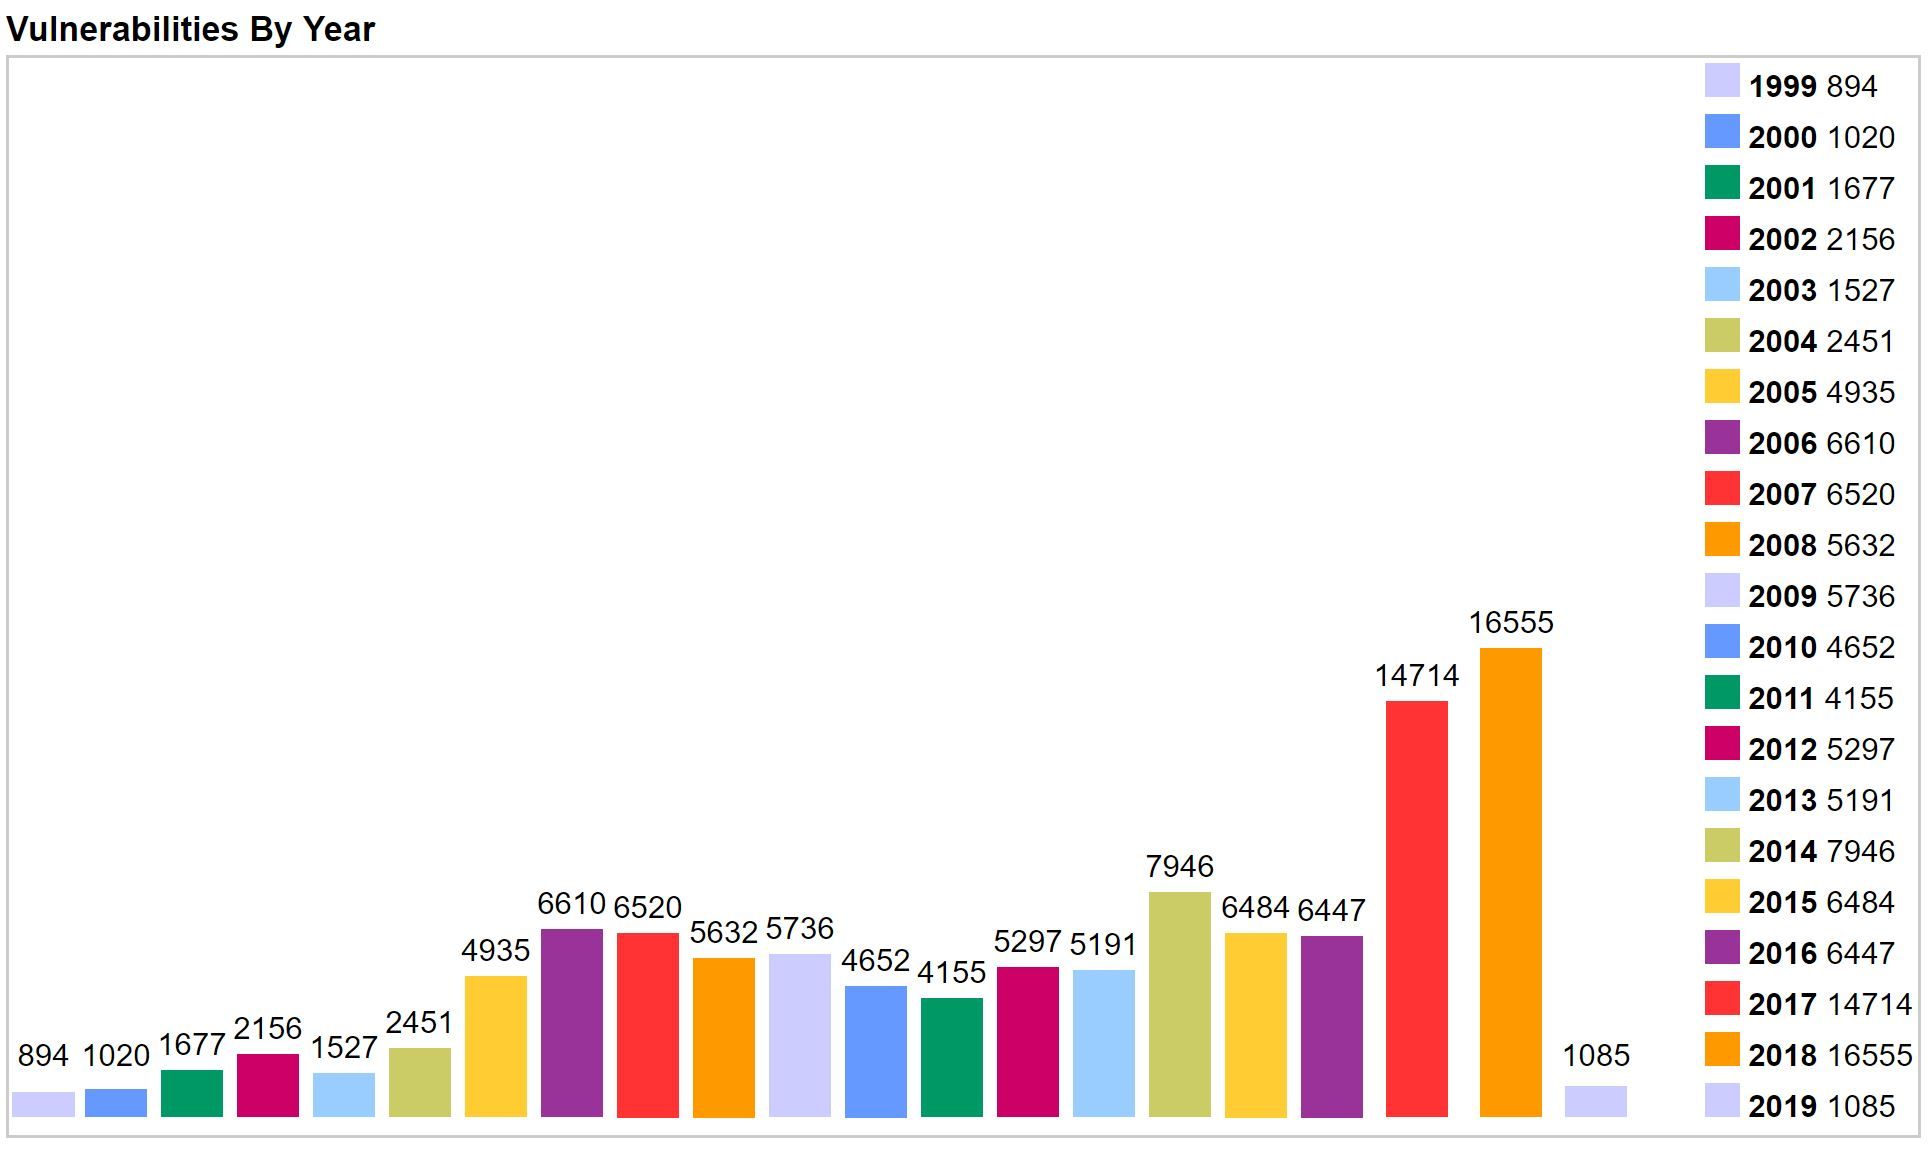
\includegraphics[width=1\textwidth]{Images/VulnByYear}
    \caption[Gefundene Schwachstellen pro Jahr laut CVE]{Gefundene Schwachstellen pro Jahr laut CVE \cite{cve}}
  \end{figure}

\chapter{Grundlagen}
  \section{Web Application Security}
    \subsection{Bedrohungen}
    TODO
      \subsubsection{OWASP Top 10}

    \subsection{Sicherheitsmaßnahmen}
    TODO

    \subsubsection{Web Application Firewalls (WAF)}
    TODO

    \subsubsection{Penetrationtesting}
    TODO

    \paragraph{Black-Box Testing}
    Beim Black-Box Testing befindet sich der Tester in der Rolle eines typischen Hackers von
    außen, der kein Wissen über die innere Arbeitsweise der Anwendung hat, weder Architektur noch
    Quellcode sind bekannt. Der Angreifer muss mit manuellen Methoden sowie speziellen Tools des Penetrationstestings vertraut sein, um Schwachstellen zu lokalisieren und auszunutzen. Für die dynamische Analyse des anzugreifenden Netzwerks benötigt er Scanning Tools, die in der vorliegenden Arbeit evaluiert werden.

    \paragraph{Grey-Box Testing}
    Während der Black-Box-Tester ein System aus der Sicht eines Außenseiters untersucht, hat ein    Grey-Box Tester bereits Zugriff auf das System auf Benutzerebene, möglicherwei- se sogar mit    erhöhten Berechtigungen eines Administrators. In der Regel liegt eine Dokumentation über Design und Architektur des Netzwerks vor, die internen Komponenten sind bekannt. Dies hat den Vorteil, dass die Sicherheit des Netzwerks gezielter und effizienter beurteilt werden kann, der Tester kann sich sofort auf die Systeme konzentrieren, die am wichtigsten sind oder ein besonders hohes Risiko haben. Zudem kann durch das interne Benutzerkonto ein Angriff innerhalb des abgesicherten Systems mit umfassendem Zugriff auf das Netzwerk simuliert werden.

    \paragraph{White-Box Testing}
    TODO
    \paragraph{Rechtliche Aspekte}
      \subparagraph{Hacker/Cracker vs. Pentester}
      TODO

  \section{Security Tools}
    \subsection{Mapping Tools}
    TODO
    \subsection{Scanning Tools}
    TODO
    \subsection{Exploitation Tools}
    TODO

\chapter{Methodik}
\section{Testverfahren}
Der Ablauf des Testens war für jeden WVS identisch.
Zunächst wurden die verwundbare Web-Applikation gescannt und ein entsprechender Bericht generiert, anhand dessen die gefundenen Schwachstellen analysiert werden konnten. Um die True und False Positives zu identifizieren war es notwendig, die gefundenen Schwachstellen manuell zu validieren und die Ergenisse zu vergleichen.
Dabei wurden stichpunktartig Notizen über Handhabung und Bedienbarkeit gemacht, teilweise bedurfte es zusätzlicher Konfiguration der WVS, um brauchbare Ergebnisse zu erhalten.

\section{Web Vulnerability Scanner (WVS)}
  \subsection{Auswahlkriterien}
  OWASP listet 50 verschiedene Tools zum Scannen von Web-Applications auf
  \cite{OWASPtools}. Die Auswahl wurde auf WVS mit folgenden Eigenschaften eingegrenzt:
  \begin{itemize}
    \item 1. Free und Open Source WVS.
    \item 2. Kommerzielle WVS, die eine Free- oder Community-Edition anbieten.
    \item 3. WVS, deren aktuelles Release nicht älter als 2 Jahre ist.
    \item 4. WVS, die in der Lage sind, umfassende Scans auszuführen, um möglichst viele verschiedene Schwachstellenarten aufzuspüren.
  \end{itemize}
  Zudem wurde bei den Firmen mit den bekanntesten kommerziellen WVS eine Trial Version angefragt, um ein realistisches Abbild der aktuell meistgenutzten Tools zu erhalten und um die Ergebnisse der kostenlosen denen der kommerziellen Scanner gegenüber zu stellen. Es handelt sich um folgende Firmen:
  \\Acunetix, Beyond Security (AVDS), Beyond Trust (Retina), Netsparker, N-Stalker, Rapid 7 (Nexpose) und Tenable (Nessus).

  \subsection{Ausgewählte WVS}
    \subsubsection{Free und Open Source WVS}
      \begin{table}[!htb]
        \begin{tabular}{|l|l|l|l|}
          \hline
          WVS              & Anbieter  & Version                      & Plattform \\ \hline
          Arachni          &           &                              &           \\ \hline
          GoLismero        &           &                              &           \\ \hline
          Grabber          &           &                              &           \\ \hline
          OpenVAS          & Greenbone &                              &           \\ \hline
          Skipfish         &           &                              &           \\ \hline
          Vega             &           &                              &           \\ \hline
          Wapiti           &           &                              &           \\ \hline
          Watobo           &           &                              &           \\ \hline
          Wfuzz            &           &                              &           \\ \hline
          W3af             &           &                              &           \\ \hline
          Zed Attack Proxy &  OWASP    &                              &           \\ \hline
          \end{tabular}
          \caption[Ausgewählte Free und Open Source WVS]{Ausgewählte Free und Open Source WVS}
        \end{table}

    \subsubsection{Kommerzielle WVS}
      \begin{itemize}
        \item BurpSuite Professional v2.0.15beta
      \end{itemize}

  \subsection{Nicht ausgewählte WVS}
    \subsubsection{Free und Open Source WVS}
    \begin{itemize}
      \item Grendel-Scan: Veraltet (Last modified 2010)
      \item Iron Wasp: Beim Downloadversuch kam die Fehlermeldung ``Down (Service unavailable)''
      \item Nikto: Nikto ist im GoLismero Bundle enthalten und bedarf daher keiner separaten Evaluation
      \item Ratproxy: Veraltet (Latest Release 2009)
      \item SQLmap: Ist auf das Auffinden von SQLi Schwachstellen begrenzt
      \item Webscarab: Veraltet (Latest Release 2011)
      \item Wikto: Ist lediglich eine Windows-Portierung von Nikto
      \item Xenotix: Ist auf das Auffinden von Cross-Site-Scripting Schwachstellen begrenzt
    \end{itemize}

    \subsubsection{Kommerzielle WVS}
      \begin{itemize}
        \item N-Stalker: Die angebotene ``7-Day Evaluation Licence'' erlaubt nur das Scannen einer einzigen, vorher festgelegten URL und ist daher für den geplanten Testaufbau nicht geeignet.
      \end{itemize}

\section{Verwundbare Web-Applikationen}
  \subsection{OWASP Juice Shop}
  TODO
  \subsection{Damn Vulnerable Web Application}
  TODO
  \subsection{WebGoat}
  WebGoat ist ein weiteres Projekt von OWASP, für diese unsichere Webanwendung gibt es für jede Schwachstelle einzelne Lektionen, in denen der Benutzer nachweisen muss, dass er ein Sicherheitsproblem verstanden hat. Benutzt wird die aktuelle Version 8.0.0.M23 vom 18.01.2019.

  \subsection{Zero Bank}
  TODO
  \subsection{Altoro Mutual}
  TODO
  \subsection{Webscantest}
  TODO
  \subsection{Security Tweets}
  TODO


\chapter{Evaluation}
  \section{Gefundene Schwachstellen per Web Application}
  TODO
  \section{Gefundene Schwachstellen nach Schwachstellentyp}
  TODO
  \section{Treffergenauigkeit}
  TODO
  \section{Bedienung und benötigter Konfigurationsumfang der WVS}
  \subsubsection{BurpSuite Pro}
  Die Firma Portswigger bietet eine 30-tägige Testversion mit allen Funktionen für BurpSuite Professional an. BurpSuite Pro enthält eine umfangreiche Dokumentation mit zahlreichen Hilfestellungen für verschiedene Anwendungsszenarien.  Das Dashboard ist sehr übersichtlich und intuitiv zu bedienen: mit Hilfe des Buttons ``New Scan'' lässt sich direkt ohne größeren Konfigurationsaufwand eine Website erfolgreich scannen.

  \begin{figure}[!htb]
    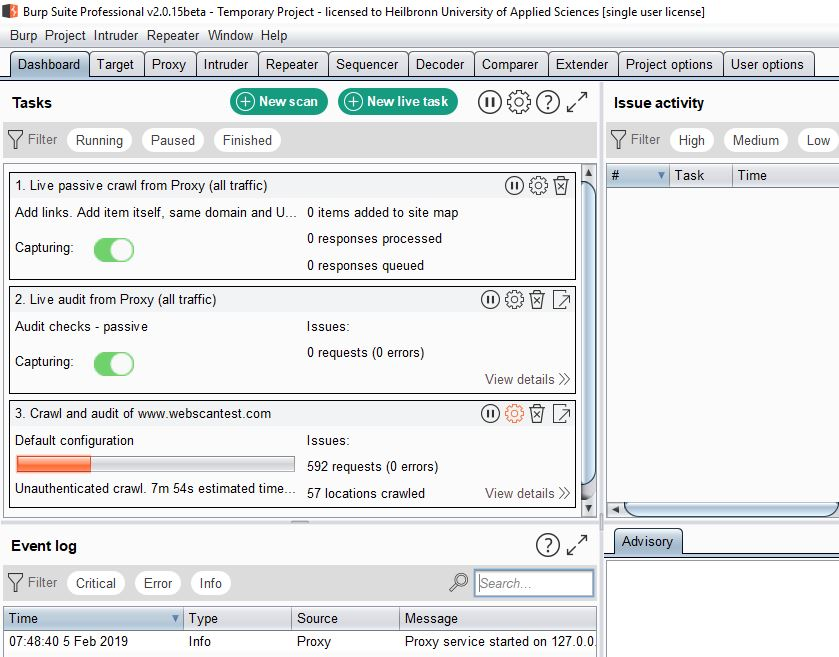
\includegraphics[width=1\textwidth]{Images/BurpSuitePro}
    \caption[Dashboard von BurpSuite Pro]{Dashboard von BurpSuite Pro}
  \end{figure}

\chapter{Diskussion}
  \section{Open Source WVS}
  TODO
  \section{Kommerzielle WVS}
  TODO
  \section{Open Source vs. kommerziell}
  TODO
  \section{Empfehlung}


\chapter{Fazit und Ausblick}
TODO
  \section{OWASP Benchmark}
  TODO


\backmatter


%%%%%%%%%%%%%%%%%%%
%% create listings list
%%%%%%%%%%%%%%%%%%%
%\lstlistoflistings
%\addcontentsline{toc}{chapter}{Listings}

\cleardoublepage
\phantomsection
\addcontentsline{toc}{chapter}{Quellenverzeichnis}
\printbibliography[title=Quellenverzeichnis]

\appendix
  \chapter*{Anhang}
  \addtocontents{toc}{\protect{\vspace{3ex}}}
  \addcontentsline{toc}{chapter}{Anhang}

  \section{Verwendete Abk"urzungen}
  \dots{}

  \section{OWASP: The Open Web Application Security Project}
  Das ``Open Web Application Security Project'' (OWASP) ist eine unabhängige, weltweite Community mit dem Ziel, die Bedeutung der Sicherheit von Webanwendungen »sichtbar zu machen«, Fachwissen zur Entwicklung und den Betrieb sicherer Webanwendungen zu verbreiten und frei zur Verfügung zu stellen.
  OWASP ist mit keinem Technologieunternehmen verbunden, obwohl der Einsatz kommerzieller Sicherheitstechnologien unterstützt wird. Sämtliche OWASP-Instrumente, wie Dokumente, Videos, Slides, Podcasts etc. sind kollaborativ produziert worden und sind zudem kostenlos unter einer freien Lizenz verwendbar. Die OWASP Foundation ist eine Non-Profit-Organisation, die sich vier Grundwerten verschrieben hat:

  \begin{itemize}
    \item Offenheit: Von den Finanzen bis zum Code ist alles radikal transparent.
    \item Innovation: OWASP fördert und unterstützt Innovationen und Experimente zur Lösung von Software-Sicherheitsherausforderungen.
    \item Globalität: Jeder auf der ganzen Welt kann sich an der OWASP-Community beteiligen.
    \item Integrität: OWASP ist eine ehrliche und aufrichtige, herstellerneutrale, globale Gemeinschaft.
  \end{itemize}

  Zudem gibt es einen Verhaltenskodex mit folgenden Prinzipien:
  \begin{itemize}
    \item Führe alle beruflichen Tätigkeiten und Pflichten in Übereinstimmung mit allen anwendbaren Gesetzen und den höchsten ethischen Grundsätzen aus.
    \item Fördere die Umsetzung von Normen, Verfahren und Kontrollen für die Anwendungssicherheit und deren Einhaltung.
    \item Bewahre eine angemessenene Vertraulichkeit gegenüber geschützter oder anderweitig sensibler Informationen, die im Rahmen einer beruflichen Tätigkeit auftreten.
    \item Übernimm die berufliche Verantwortung mit Sorgfalt und Ehrlichkeit.
    \item Kommuniziere offen und ehrlich.
    \item Vermeide Aktivitäten, die einen Interessenskonflikt hervorrufen oder anderweitig den Ruf des Arbeitgebers, den Informationssicherheitsberuf oder die Vereinigung beeinträchtigen könnten.
    \item Bewahre und verstärke unsere Objektivität und Unabhängigkeit.
    \item Weise unangemessenen Druck der von Seiten der Industrie oder anderen zurück.
    \item Verletze oder bestreite nicht absichtlich den Ruf von Kollegen, Kunden oder Arbeitgebern.
    \item Behandle jeden mit Respekt und Würde.
    \item Vermeide Beziehungen, die die Objektivität und Unabhängigkeit von OWASP  beeinträchtigen könnten.
  \end{itemize}

\cite{OWASPabout}

    \subsection{Die OWASP Top Ten}
    TODO
\cite{OWASPtop10}

    \subsubsection{A1: Injection}
    Injection-Schwachstellen, wie beispielsweise SQL-, OS- oder LDAP-Injection, treten auf, wenn
    nicht vertrauenswürdige Daten von einem Interpreter als Teil eines Kommandos oder einer
    Abfrage verarbeitet werden. Ein Angreifer kann Eingabedaten dann so manipulieren, dass er nicht
    vorgesehene Kommandos ausführen oder unautorisiert auf Daten zugreifen kann.

    \subsubsection{A2: Fehler in der Authentifizierung}
    Anwendungsfunktionen, die im Zusammenhang mit Authentifizierung und Sessionmanagement
    stehen, werden häufig fehlerhaft implementiert. Dies erlaubt es Angreifern, Passwörter oder
    Session-Token zu kompromittieren oder die entsprechenden Schwachstellen so auszunutzen,
    dass sie die Identität anderer Benutzer vorübergehend oder dauerhaft annehmen können.

    \subsubsection{A3: Verlust der Vertraulichkeit sensibler Daten}
    Viele Anwendungen schützen sensible Daten, wie personenbezogene Informationen und Finanzoder
    Gesundheitsdaten, nicht ausreichend. Angreifer können diese Daten auslesen oder
    modifizieren und mit ihnen weitere Straftaten begehen (Kreditkartenbetrug, Identitätsdiebstahl
    etc.). Vertrauliche Daten können kompromittiert werden, wenn sie nicht durch Maßnahmen, wie
    Verschlüsselung gespeicherter Daten und verschlüsselte Datenübertragung, zusätzlich geschützt
    werden. Besondere Vorsicht ist beim Datenaustausch mit Browsern angeraten.

    \subsubsection{A4: XML External Entities}
    Viele veraltete oder schlecht konfigurierte XML Prozessoren berücksichtigen Referenzen auf
    externe Entitäten innerhalb von XML-Dokumenten. Dadurch können solche externen Entitäten
    dazu eingesetzt werden, um mittels URI Datei-Handlern interne Dateien oder File-Shares offenzulegen
    oder interne Port-Scans, Remote-Code-Executions oder Denial-of-Service Angriffe
    auszuführen.

    \subsubsection{A5: Fehler in der Zugriffskontrolle}
    Häufig werden die Zugriffsrechte für authentifizierte Nutzer nicht korrekt um- bzw. durchgesetzt.
    Angreifer können entsprechende Schwachstellen ausnutzen, um auf Funktionen oder Daten
    zuzugreifen, für die sie keine Zugriffsberechtigung haben. Dies kann Zugriffe auf Accounts
    anderer Nutzer sowie auf vertrauliche Daten oder aber die Manipulation von Nutzerdaten,
    Zugriffsrechten etc. zur Folge haben.

    \subsubsection{A6: Sicherheitsrelevante Fehlkonfiguration}
    Fehlkonfigurationen von Sicherheitseinstellungen sind das am häufigsten auftretende Problem.
    Ursachen sind unsichere Standardkonfigurationen, unvollständige oder ad-hoc durchgeführte
    Konfigurationen, ungeschützte Cloud-Speicher, fehlkonfigurierte HTTP-Header und Fehlerausgaben,
    die vertrauliche Daten enthalten. Betriebssysteme, Frameworks, Bibliotheken und Anwendungen
    müssen sicher konfiguriert werden und zeitnah Patches und Updates erhalten.

    \subsubsection{A7: Cross-Site-Scripting (XSS)}
    XSS tritt auf, wenn Anwendungen nicht vertrauenswürdige Daten entgegennehmen und ohne
    Validierung oder Umkodierung an einen Webbrowser senden. XSS tritt auch auf, wenn eine
    Anwendung HTML- oder JavaScript-Code auf Basis von Nutzereingaben erzeugt. XSS erlaubt es
    einem Angreifer, Scriptcode im Browser eines Opfers auszuführen und so Benutzersitzungen zu
    übernehmen, Seiteninhalte verändert anzuzeigen oder den Benutzer auf bösartige Seiten
    umzuleiten.

    \subsubsection{A8: Unsichere Deserialisierung}
    Unsichere, weil unzureichend geprüfte Deserialisierungen können zu Schwachstellen in der
    Remote-Code-Execution führen. Aber auch wenn das nicht der Fall ist, können
    Deserialisierungsfehler Angriffsmuster wie Replay-Angriffe, Injections und Erschleichung
    erweiterter Zugriffsrechte ermöglichen.

    \subsubsection{A9: Nutzung von Komponenten mit bekannten Schwachstellen}
    Komponenten wie Bibliotheken, Frameworks etc. werden mit den Berechtigungen der zugehörigen
    Anwendung ausgeführt. Wird eine verwundbare Komponente ausgenutzt, kann ein solcher
    Angriff von Datenverlusten bis hin zu einer Übernahme des Systems führen. Applikationen und
    APIs, die Komponenten mit bekannten Schwachstellen einsetzen, können Schutzmaßnahmen
    unterlaufen und so Angriffe mit schwerwiegenden Auswirkungen verursachen.

    \subsubsection{A10: Unzureichendes Logging und Monitoring}
    Unzureichendes Logging und Monitoring führt zusammen mit fehlender oder uneffektiver Reaktion auf Vorfälle zu andauernden oder wiederholten Angriffen. Auch können Angreifer dadurch in Netzwerken weiter vordringen und Daten entwenden, verändern oder zerstören. Viele Studien zeigen, dass die Zeit bis zur Aufdeckung eines Angriffs bei ca. 200 Tagen liegt sowie typischerweise durch Dritte entdeckt wird und nicht durch interne Überwachungs- und Kontrollmaßnahmen.

\cite{OWASPtop10}







%%%%%%%%%%%%%%%%%%%
%% declaration on oath
%%%%%%%%%%%%%%%%%%%

\addchap{Eidesstattliche Erklärung}

Hiermit versichere ich, dass ich die vorgelegte Bachelorarbeit selbstständig verfasst und noch nicht anderweitig zu Prüfungszwecken vorgelegt habe. Alle benutzten Quellen und Hilfsmittel sind angegeben, wörtliche und sinngemäße Zitate wurden als solche gekennzeichnet.

\vspace{20pt}
\begin{flushright}
$\overline{~~~~~~~~~~~~~~~~~\mbox{\BaAuthor, am \today}~~~~~~~~~~~~~~~~~}$
\end{flushright}


\begin{lstlisting}[label=lst:java,
				   language=java,
				   firstnumber=1,
				   caption=Beispiel für einen Quelltext]

public void foo() {
	// Kommentar
}
\end{lstlisting}

\end{document}
